% Draft of the model figure in the style of Altabaa & Lafferty (arXiv 2607.17674), Figure 2:
% tokens at the bottom, the backbone as one wide bar, states above it, one accent color for the latent,
% the training-only part in a dashed box.   Build:  tectonic model_figure.tex
% Needs TikZ with the arrows.meta, positioning, calc, fit and backgrounds libraries.
\documentclass[tikz,border=6pt]{standalone}
\usepackage{amsmath,amssymb,bm}
\usetikzlibrary{arrows.meta,positioning,calc,fit,backgrounds}

\definecolor{barfill}{HTML}{E9F0F9}   % backbone
\definecolor{barline}{HTML}{AFC1D9}
\definecolor{ink}{HTML}{3A4654}       % text and neutral lines
\definecolor{soft}{HTML}{9AA7B5}      % faded parts
\definecolor{acc}{HTML}{D55E00}       % the adapter residual (Delta h in every figure of the paper)
\definecolor{accfill}{HTML}{FCE9DC}
\definecolor{hc}{HTML}{0072B2}        % the adapter result (h in every figure of the paper)
\definecolor{trainfill}{HTML}{F6F3EC} % training-only box
\definecolor{trainline}{HTML}{C9B98F}

\newcommand{\dH}{\Delta\bm h}
\newcommand{\hon}{\bm h_{\mathrm{on}}}
\newcommand{\hoff}{\bm h_{\mathrm{off}}}

\tikzset{
  every node/.style={font=\sffamily\scriptsize, text=ink},
  adapted/.style={draw=acc!55, line width=0.8pt},
  bar/.style={draw=barline, fill=barfill, rounded corners=3pt, minimum height=6.6mm, inner sep=0pt, line width=0.5pt},
  tok/.style={draw=soft, fill=white, rounded corners=1.5pt, minimum width=7.6mm, minimum height=4.4mm, inner sep=1pt, line width=0.4pt},
  hid/.style={draw=barline, fill=barfill!55, rounded corners=1.5pt, minimum width=7.6mm, minimum height=4.4mm, inner sep=1pt, line width=0.4pt},
  key/.style={hid, draw=ink, fill=white, line width=0.6pt},
  lat/.style={draw=acc, fill=accfill, rounded corners=2pt, minimum height=5.6mm, inner sep=3pt, line width=0.7pt, text=acc!70!black},
  flow/.style={-{Stealth[length=1.5mm,width=1.2mm]}, draw=soft, line width=0.45pt},
  main/.style={-{Stealth[length=1.9mm,width=1.5mm]}, draw=acc, line width=0.8pt},
  note/.style={font=\sffamily\tiny, text=soft},
}

% a small histogram: a predictive distribution
\newcommand{\dist}[2]{% #1 position, #2 color
  \begin{scope}[shift={(#1)}]
    \foreach \x/\h in {-0.21/0.12, -0.07/0.30, 0.07/0.20, 0.21/0.08}
      \fill[#2] (\x-0.055,0) rectangle (\x+0.055,\h);
    \draw[#2, line width=0.3pt] (-0.3,0) -- (0.3,0);
  \end{scope}}

\begin{document}
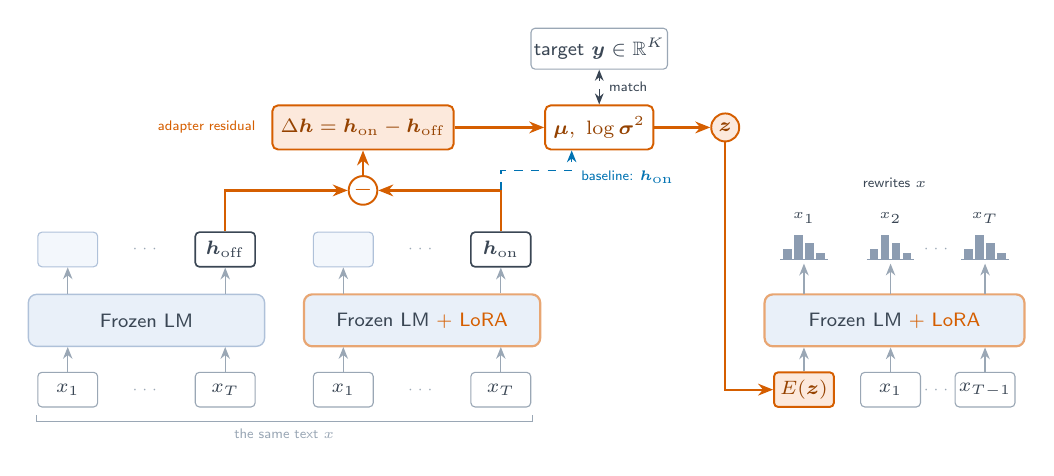
\begin{tikzpicture}[x=1cm,y=1cm]

% ---------------------------------------------------------------- encoder: two passes over the same text
\node[bar, minimum width=30mm] (Boff) at (1.5,1.3) {Frozen LM};
\node[bar, adapted, minimum width=30mm] (Bon) at (5.0,1.3) {Frozen LM \textcolor{acc}{+ LoRA}};

\foreach \bx/\name in {0/a, 3.5/b} {
  \node[tok] (\name1) at (\bx+0.5,0.42) {$x_1$};
  \node[note] at (\bx+1.5,0.42) {$\cdots$};
  \node[tok] (\name3) at (\bx+2.5,0.42) {$x_T$};
  \node[hid] (\name h1) at (\bx+0.5,2.2) {};
  \node[note] at (\bx+1.5,2.2) {$\cdots$};
  \foreach \i in {1,3} \draw[flow] (\name\i.north) -- (\name\i.north |- Boff.south);
  \draw[flow] (\name h1.south |- Boff.north) -- (\name h1.south);
}
\node[key] (hoff) at (2.5,2.2) {$\hoff$};
\node[key] (hon)  at (6.0,2.2) {$\hon$};
\draw[flow] (hoff.south |- Boff.north) -- (hoff.south);
\draw[flow] (hon.south |- Bon.north) -- (hon.south);
\draw[soft, line width=0.4pt] (0.1,0.1) -- (0.1,0.02) -- (6.4,0.02) -- (6.4,0.1);
\node[note, below] at (3.25,0.04) {the same text $x$};

% ---------------------------------------------------------------- the adapter residual and the latent
\node[circle, draw=acc, fill=white, inner sep=0.6pt, line width=0.7pt, text=acc, font=\sffamily\footnotesize] (minus) at (4.25,2.95) {$-$};
\draw[main] (hoff.north) |- (minus.west);
\draw[main] (hon.north) |- (minus.east);
\node[lat] (dh) at (4.25,3.75) {$\dH = \hon - \hoff$};
\draw[main] (minus) -- (dh);
\node[note, text=acc, anchor=east] at ($(dh.west)+(-0.08,0)$) {adapter residual};

\node[lat, fill=white] (mu) at (7.25,3.75) {$\bm\mu,\ \log\bm\sigma^2$};
\draw[main] (dh) -- (mu);
% the baseline readout
\draw[-{Stealth[length=1.5mm,width=1.2mm]}, hc, dashed, line width=0.5pt] (6.0,2.95) |- (6.9,3.2) -- (6.9,3.2 |- mu.south);
\node[note, text=hc, anchor=west, inner sep=1pt] at (6.98,3.12) {baseline: $\hon$};

% the alignment target
\node[tok, minimum width=17mm, minimum height=5.2mm] (y) at (7.25,4.75) {target $\bm y \in \mathbb R^{K}$};
\draw[{Stealth[length=1.4mm,width=1.1mm]}-{Stealth[length=1.4mm,width=1.1mm]}, draw=ink, dashed, line width=0.45pt] (mu) -- node[note, right, text=ink]{match} (y);

\node[circle, draw=acc, fill=accfill, inner sep=1.6pt, line width=0.7pt, text=acc!70!black] (z) at (8.85,3.75) {$\bm z$};
\draw[main] (mu) -- (z);

% ---------------------------------------------------------------- generator
\node[bar, adapted, minimum width=33mm] (Bgen) at (11.0,1.3) {Frozen LM \textcolor{acc}{+ LoRA}};
\node[tok, draw=acc, fill=accfill, text=acc!70!black, line width=0.7pt] (ez) at (9.85,0.42) {$E(\bm z)$};
\node[tok] (g1) at (10.95,0.42) {$x_1$};
\node[note] at (11.55,0.42) {$\cdots$};
\node[tok] (g3) at (12.15,0.42) {$x_{T-1}$};
\foreach \n in {ez,g1,g3} \draw[flow] (\n.north) -- (\n.north |- Bgen.south);
\draw[main] (z.south) |- (ez.west);
\foreach \x/\lab in {9.85/{x_1}, 10.95/{x_2}, 12.15/{x_T}} {
  \draw[flow] (\x,1.64) -- (\x,2.02);
  \dist{\x,2.08}{barline!70!ink}
  \node[note, text=ink] at (\x,2.6) {$\lab$};
}
\node[note] at (11.55,2.2) {$\cdots$};
\node[note, text=ink] at (11.0,3.05) {rewrites $x$};

\end{tikzpicture}
\end{document}
